Si vous travaillez sur un système d'exploitation sous Linux, nous allons vous expliquer dans cette partie comment compiler et lancer le projet.

Tout d'abord, positionnez-vous dans le dossier "Projet-INFO0503" comme ceci : 

\begin{figure}[h]
    \centering
    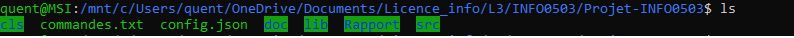
\includegraphics[width= 170mm, height=10mm]{images/positionnement.png}
    \caption{Positionnement dans le dossier}
    \label{img:mesh1}
\end{figure}

Puis réaliser la compilation de l'ensemble des fichiers en utilisant la commande suivante : \newline
\textbf{javac -d cls/ -cp lib/json-20220924.jar -sourcepath src/ src/Lanceur.java}

\begin{figure}[h]
    \centering
    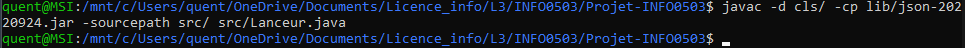
\includegraphics[width= 170mm, height=10mm]{images/compilation.png}
    \caption{Succès de la compilation}
    \label{img:mesh2}
\end{figure}

Une fois la compilation terminée, vous pouvez donc lancer le projet en utilisant la commande suivante : \newline
\textbf{java -cp cls/:lib/json-20220924.jar Lanceur config.json} \newline
Il se peut que vous ayez un message d'erreur comme vous pouvez le voir sur la figure ci-dessous au moment du lancement de vos serveur HTTP.
\begin{figure}[h]
    \centering
    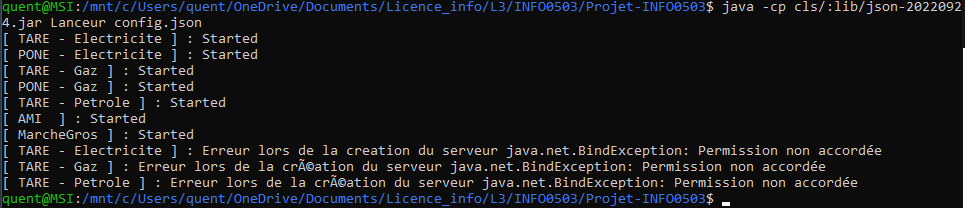
\includegraphics[width= 170mm, height=40mm]{images/erreurLancement.png}
    \caption{Erreur de lancement}
    \label{img:mesh3}
\end{figure}
\newpage
Pour résoudre ce probléme, il vous suffit de passer en superadmin en utilsant le préfixe \textbf{sudo}, comme ceci : \newline
\textbf{sudo java -cp cls/:lib/json-20220924.jar Lanceur config.json}
\begin{figure}[h]
    \centering
    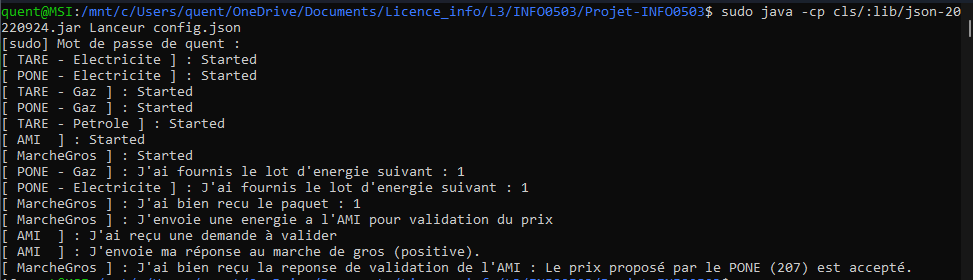
\includegraphics[width= 170mm, height=60mm]{images/succesLancement.png}
    \caption{Succès du lancement}
    \label{img:mesh4}
\end{figure}

Nous voila avec le projet opérationnel du côté serveur. Si le serveur PHP est également opérationnel, vous avez juste à vous rendre dans votre nativateur web et rentrer \textbf{localhost} dans la barre de recherche. Vous pouvez commencer à faire vos simulations d'achat d'énergie, et en même temps consulter les différentes communications entre toutes les entités dans le terminal. Vous pouvez alors essayer les différents sénarios ainsi que créer vos propres commandes.
\begin{figure}[h]
    \centering
    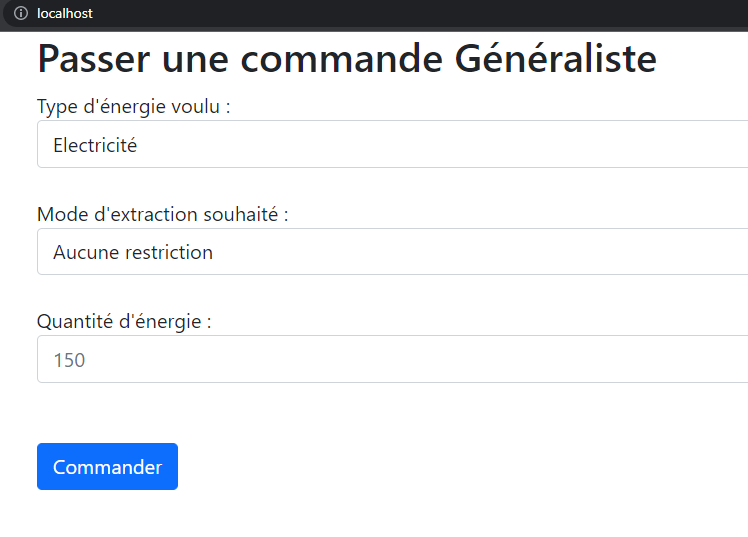
\includegraphics[width= 85mm, height=60mm]{images/Localhost.png}
    \caption{Interface WEB}
    \label{img:mesh5}
\end{figure}
\newpage